Snapchat ist eine kostenlose Smartphone Anwendung f\"ur Android und iOS, die es
seinen Nutzern erm\"oglicht Bild- sowie Videonachrichten zu versenden. Die App
wurde im September 2011 initial released und ist mittlerweile in $20$ Sprachen
\"ubersetzt. Im Gegensatz zu YouNow gibt es f\"ur Snapchat keine
Desktopvariante.

Eine Besonderheit gegen\"uber anderen Anwendungen ist, dass die Medieninhalte
nur f\"ur begrenzte Zeit, d.h. mindestens eine und maximal $10$ Sekunden
f\"ur den/die Empf\"anger sichtbar sind. Nach diesem Zeitraum l\"oschen sich
,laut Anbieter, die Dateien von selbst beim Client. Mittlerweile ist es jedoch
m\"oglich die Inhalte mehrfach anzusehen. Zudem kann ein Nutzer eine sogenannte
,,Snapchat-Geschichte'' anlegen, welche $24$ Stunden sichtbar und mit
bestimmten Freunden oder der gesamten Community teilbar ist.

\paragraph{Anmeldung}
Bevor man die Anwendung auf seinen Smartphone installieren kann, muss man
Snapchat umfangreiche Rechte zugestehen. Abbildung~\ref{fig:sc_perms} zeigt
examplarisch die Rechteanfordungen unter Android.
\begin{figure}[ht]
	\centering
	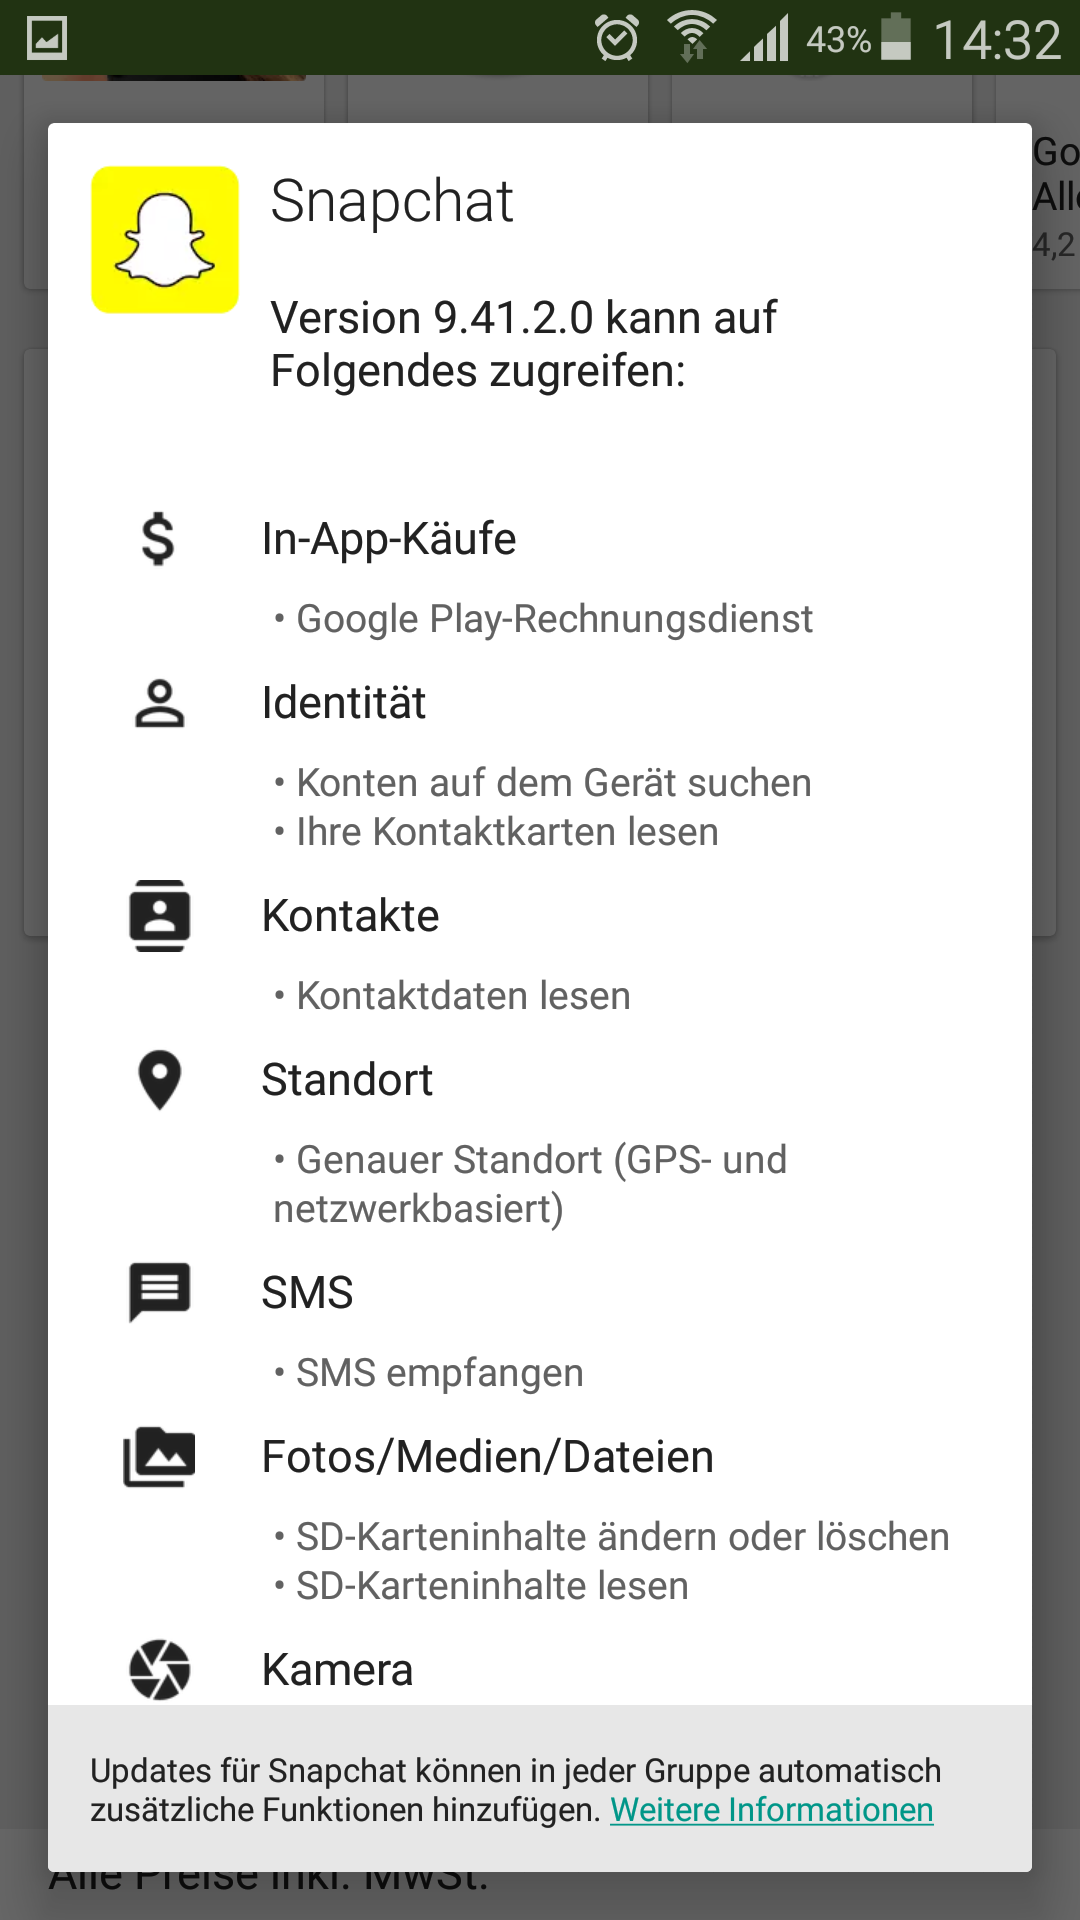
\includegraphics[width=0.4\linewidth]{resources/sc_perms_1.png}
	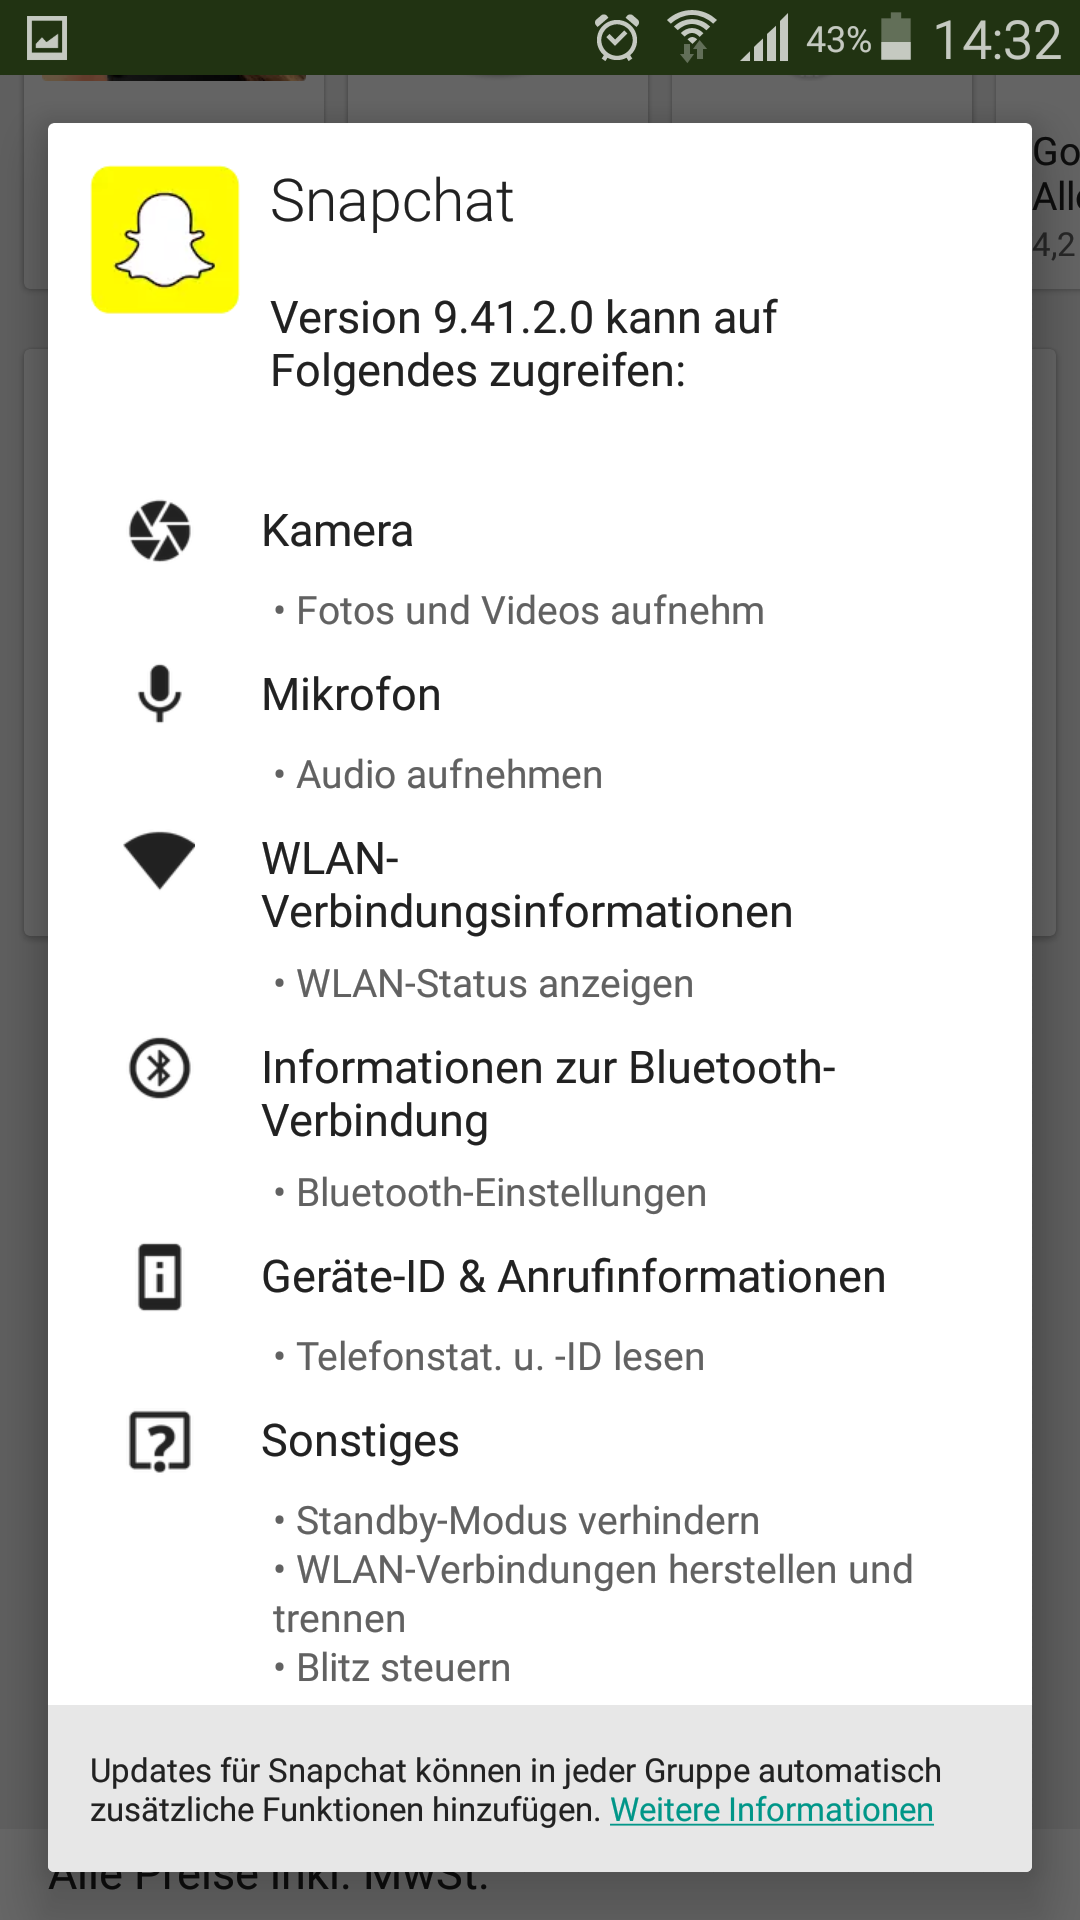
\includegraphics[width=0.4\linewidth]{resources/sc_perms_2.png}
	\label{fig:sc_perms}
	\caption{\"Ubersicht der Rechteanforderung von Snapchat auf einem Android
	Smartphone.}
\end{figure}
Unter anderem muss der App das Auslesen s\"amtlicher Kontakt- sowie
Standortdaten des Ger\"ats gew\"ahrleistet werden. Auch der Zugriff auf
Fotos, Videos, Medien sowie Kamera und Mikrofon muss freigegeben werden.

Ist die App auf dem Ger\"at installiert kann man sich als Nutzer anmelden.
Hierf\"ur ist eine Email-Adresse, ein Nutzername, das Geburtsdatum, sowie ein
Passwort erforderlich. Eine Kontrolle des Alters wird vom Anbieter nicht
durchgef\"uhrt.

\paragraph{Funktionsweise und Kommunikation}
In diesem Abschnitt m\"ochten wir noch etwas genauer auf die Funktionsweise und
Kommunikation von Snapchat eingehen.

Um \"uberhaupt Inhalte zu Versenden braucht der neu angemeldete Nutzer Personen
mit denen er kommunizieren kann. Diese kann er \"uber folgende M\"oglichkeiten
hinzuf\"ugen:
\begin{itemize}
	\item Nutzernamen: Eingabe konkreter Nutzer.
	\item Aus Kontakten: Kontaktliste des Smartphones nach Personen mit
	Snapchat durchsuchen lassen.
	\item Snapcode: Vergleichbar mit QR-Codes.
	\item In der N\"ahe: Nutzer, die im gleichen Wlan-Netz sind.
\end{itemize}

Jetzt hat der Nutzer die M\"oglichkeit sogenannte \emph{Snaps} d.h. Fotos oder
Videos aufzunehmen bzw. aus der Gallerie zu entnehmen und diese mit Text,
Filtern, etc. zu bearbeiten. Anschliessend kann er diese an seine Freunde
schicken. Wie eingangs erw\"ahnt, kann er nun auch festlegen, wie lange das
Medium auf dem Ger\"at des Empf\"angers sichtbar bleibt (eine bis max. zehn
Sekunden). Nach diesem Zeitraum wird das Datum vom Endger\"at gel\"oscht. Zudem
hat er die M\"oglichkeit das Medium seiner eigenen \emph{Geschichte} (engl.:
\emph{story}) hinzuzuf\"ugen damit es $24$ Stunden sichtbar bleibt. Von dort
aus kann er seine Snaps mit Freunden oder mit der ganzen Community teilen. Die
Inhalte k\"onnen dann von allen Beteiligten gespeichert werden.

Neben der M\"oglichkeit seinen Partnern Text-, Bild- und Snapnachrichten zu
schicken, bietet Snapchat auch einen Videochat an. Hier kann man sich in
Echtzeit mit seinem Gegen\"uber mit Hilfe seiner Smartphonekamera unterhalten.
